% AMS dept HW template example
% v0.04 by Eric J. Malm, 10 Mar 2005
\documentclass[11pt,a4paper,boxed]{caspset}

% set 1-inch margins in the document
\usepackage[left=1in,right=1in,top=1.2in,bottom=1in]{geometry}
%\usepackage{hyperref}
\usepackage{lastpage}
% include this if you want to import graphics files with /includegraphics
\usepackage{graphicx}
\usepackage{amsmath,amsfonts,amssymb}
\usepackage{setspace}
\usepackage{fancyhdr}
\usepackage{lastpage}
\usepackage{extramarks}
\usepackage{chngpage}
\usepackage{soul}
\usepackage[usenames,dvipsnames]{color}
\usepackage{graphicx,float,wrapfig}
\usepackage{ifthen}
\usepackage{listings}
\usepackage{courier}
\usepackage{multimedia}
\usepackage[toc,page,title,titletoc,header]{appendix}
\usepackage{indentfirst}
%%%%%%%%%%%%%%%%%%%%%%%%%%%%%%%%%%%%%%%%%%%%%%%%%%%%%%
\usepackage{xeCJK}
%\usepackage{fontspec}
\setCJKmainfont[BoldFont=simhei.ttf]{simsun.ttf}
%\setCJKsansfont{simhei.ttf}
%\setCJKmonofont{simfang.ttf}

%\setCJKmainfont{Adobe Song Std}
%\setCJKmainfont[BoldFont=Adobe Heiti Std]{Adobe Song Std}
%%%%%%%%%%%%%%%%%%%%%%%%%%%%%%%%%%%%%%%%%%%%%%%%%%%%%%

\graphicspath{{figures/}}
% Homework Specific Information
\renewcommand\refname{\bf 参考文献}
\renewcommand\contentsname{\bf 目 \ \ \ 录}
\renewcommand\figurename{\bf 图}
\renewcommand\tablename{\bf 表}
\renewcommand\appendixname{\bf 附录}
\renewcommand{\appendixpagename}{附录}

%\newtheorem{dingyi}{\bf 定义~}[section]
%\newtheorem{dingli}{\bf 定理~}[section]
%\newtheorem{yinli}[dingli]{\bf 引理~}
%\newtheorem{tuilun}[dingli]{\bf 推论~}
%\newtheorem{mingti}[dingli]{\bf 命题~}


\newcommand{\hmwkTitle}{现代物理问题的计算机模拟}
\newcommand{\hmwkSubTitle}{} % No subtitle, so this will be excluded
\newcommand{\hmwkDueDate}{11/02/2011}
\newcommand{\hmwkClass}{物理学院}
\newcommand{\hmwkClassTime}{Thu/Fri{~}8:00}
\newcommand{\hmwkClassInstructor}{周昕}
\newcommand{\hmwkAuthorName}{周吕文}

%\hypersetup{pdfauthor={\hmwkAuthorName}, 
%            pdftitle={网格渗透(percolation)过程的模拟}, 
%            pdfsubject={\hmwkTitle, \hmwkClassInstructor},
%            pdfkeywords={计算物理},
%            pdfproducer={XeLateX with hyperref},
%            pdfcreator={Xelatex}}

%% Setup the header and footer
\pagestyle{fancy}                                                       %
\lhead{\hmwkAuthorName}                                                 %
\chead{\hmwkClass\ (\hmwkClassInstructor): \hmwkTitle}  %
\rhead{第\ \thepage\ 页,{~} 共\ \protect\pageref{LastPage} 页}          %                                %
\definecolor{DarkGreen}{rgb}{0.0,0.45,0.0}

%%%%%%%%%%%%%%%%%%%%%%%%%%%%%%%%%%%%%%%%%%%%%%%%%%%%%%%%%%%%%

\setlength{\parskip}{5pt}
%%%%%%%%%%%%%%%%%%%%%%%%%%%%%%%%%%%%%%%%%%%%%%%%%%%%%%%%%%%%%

\usepackage{palatino}
\usepackage{listings} % Gives syntax highlighting for python code.
\usepackage{color} % Used for syntax highlighting.
\usepackage{textcomp} % Used for syntax highlighting.

% This gives syntax highlighting in the python environment
\renewcommand{\lstlistlistingname}{Code Listings}
\renewcommand{\lstlistingname}{Code Listing}
\definecolor{gray}{gray}{0.5}
\definecolor{key}{rgb}{0,0.5,0}
\lstnewenvironment{python}[1][]{
\lstset{
language=python,
basicstyle=\ttfamily\small,
otherkeywords={1, 2, 3, 4, 5, 6, 7, 8 ,9 , 0, -, =, +, [, ], (, ), \{, \}, :, *, !},
keywordstyle=\color{blue},
stringstyle=\color{red},
showstringspaces=false,
emph={class, pass, in, for, while, if, is, elif, else, not, and, or,
def, print, exec, break, continue, return},
emphstyle=\color{black}\bfseries,
emph={[2]True, False, None, self},
emphstyle=[2]\color{key},
emph={[3]from, import, as},
emphstyle=[3]\color{blue},
upquote=true,
morecomment=[s]{"""}{"""},
commentstyle=\color{gray}\slshape,
framexleftmargin=1mm, framextopmargin=1mm, frame=shadowbox,
rulesepcolor=\color{blue},#1
}}{}



% info for header block in upper right hand corner
\name{周吕文{~}201128000718065}
\class{物理学院{~}20110308班}
\assignment{Project \# 01}
\duedate{11/24/2011}


\begin{document}

\problemlist{\LARGE\bf 网格渗透(percolation)过程的模拟}
\section{引言}
渗透理论(percolation theory)是一个简单的相变模型. 在物理研究中的应用越来越广泛, 许多研究者活跃于这一理论. 渗透理论研究的是渗透物在随机介质中能否通过. 一个典型的例子就是渗流, 假想某种液体从一个多孔介质的顶部渗入, 那么液体能否通过一个个的孔洞, 最终到达多孔介质的底部呢? 更形象的例子有
\begin{itemize}
\item 一片干草地, 火焰从一块干草区域开始烧, 火焰能够通过整个区域的概率是多少?
\item 随机的由绝缘和金属材料组成的系统, 系统能够导电的概率是多少?
\item 假设不考虑人口的迁移, 流行病能从一个区域传到另一个区域的概率是多少?
\end{itemize}

渗透理论的研究, 促进了对其它许
多物理系统的理解, 涉及生物, 物理, 地理等等. 同时渗透理论也有很重要的实际应用, 如油的回收. 本文将考虑最简单的情况即二维方网格下的渗透模型, 及其计算机模拟的实现.

\section{二维方网格渗透模型}
数学上, 渗透理论描述的是随机图中的联通集群问题. 引言中的几个例子可以被描述为含$n\times n$(或$n\times n\times n$)个节点的二维(三维)方形网络, 相邻节点间以$p$的概率联通, 并且节点与节点间是否联通是相互独立的, 对于这样一个系统, 给定系统的尺度$n$及概率$p$, 从顶部到底部的至少存在一条通路的概率$q$是多少呢? 这个问题是由Broadbent和Hammersley于1957年
首先提出的.

这个问题还可以被进一步扩展, 考虑一个无限大的系统($n\rightarrow\infty$), 是否存在一个由开放节点组成的无穷长的通路, 或者称开放群集(open cluster).
零一定律(Kolmogorov's zero-one law)指出, 对于给定的$p$, 无限大的开放群集存在的概率要么几乎是1, 要么几乎是0. 然而,存在的概率是$p$的一个不减函数。因此必然存在一个临界值$p_c$,
在$p<p_c$是, 无限大开放群集存在的概率为0,
在$p>p_c$是, 无限大开放群集存在的概率为1. 实际上, 即使在系统尺度$n$较小时,如$n=100$, 存在一条从顶部到底部通路的概率从0到1的变化也已经相当急剧. 对于有些问题, $p_c$存在精确的理论解. 比如二维方网格, 其相变的概率临界值$p_c=1/2$. 这是由Kesten于1982给出的. 也有些问题不能给出精确的理论解, 如二维超立方网格.

在本文中, 渗透模型被限制于二维方网格中. 将介质看为一系列的二维网格, 那么渗透问题及引言中三个例子可抽像为图\ref{percolation}所示的问题, 即由开放点(open site)和阻碍点(blocked site)组成的系统, 每个网格以一定的概率$p$为开放点(下文简称点开放概率$q$). 能找到一条从顶端到底端完全由开放点构成的不间断通路的概率$q$(下文简称渗透概率$q$)是多少?
图\ref{percolation}中:
\begin{itemize}
\item \textbf{左图}: 系统大小为$n=8$, 点开放概率$p=0.6$. 存在从顶部到底部由开放点构成的不间断通路, 即产生了渗透.
\item \textbf{右图}: 系统大小为$n=8$, 点开放概率$p=0.5$. 不存在从顶部到底部由开放点构成的不间断通路, 即不能渗透.
\end{itemize}
\begin{figure}[!htb]
\centering
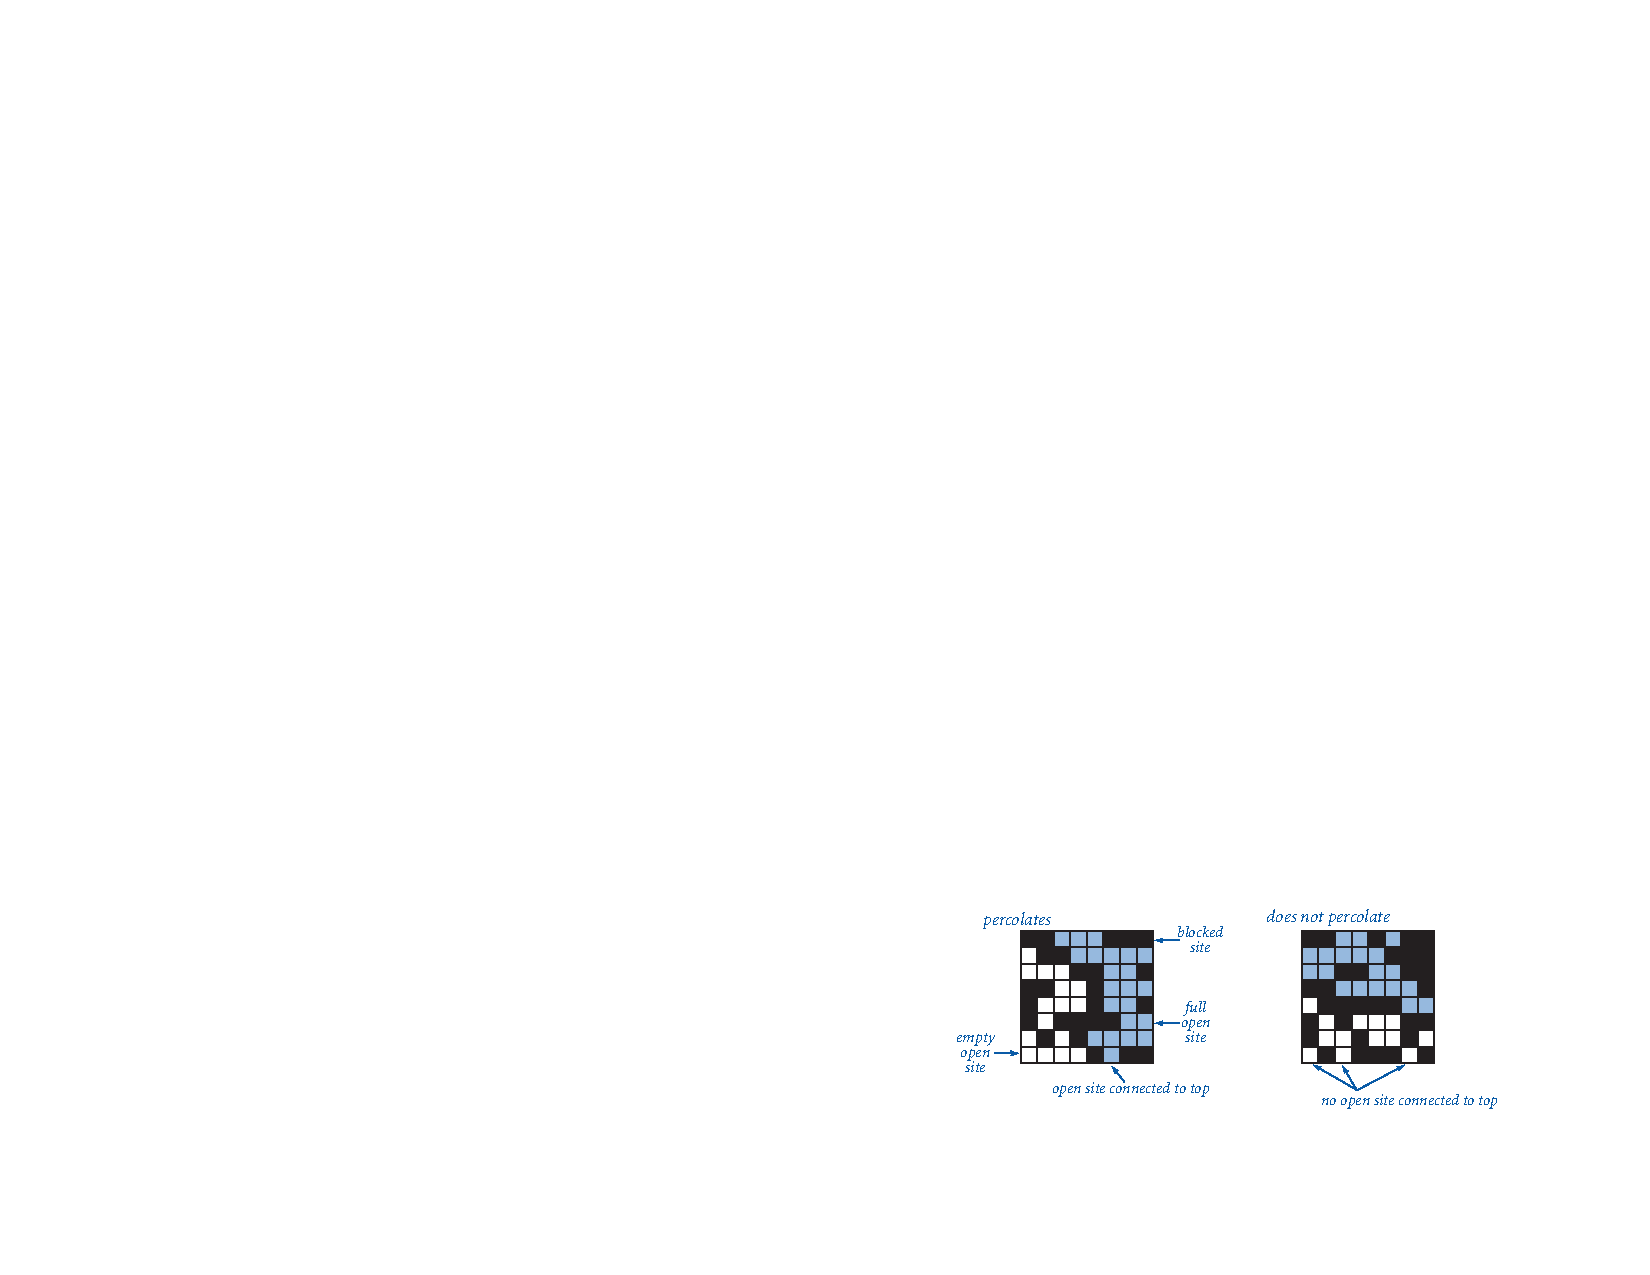
\includegraphics[width=0.85\textwidth]{fig01.pdf}
\caption{\label{percolation}渗透问题中渗透和不渗透示意图}
\end{figure}

\section{计算机模拟}
对于给定系统大小$n$, 点开放概率$p$的网格, 其渗透概率$q$可通过多次实验后的频率来近似. 基于这个想法, 本文用计算机做多次随机实验来给出不同尺度大小, 不同点开放概率下系统的渗透概率. 因此, 问题的关键在于随机渗透实验的计算机实现. 一次计算机随机渗透实验主要需要完成以下两个步骤:
\begin{enumerate}
\item 以矩阵或数组表示网格, 以1表示开放点, 0表示阻碍点. 初始化矩阵, 每个位置以概率$p$为1, $1-p$的概率为0.
\item 搜索矩阵中是否存在从首行到尾行由1构成的通路.
\end{enumerate}
下面, 分别来描述本文对于以上两个步骤的具体实现方式.

\subsection{渗流网格的初始化}
本文对渗流网格(矩阵)的初始化提供两种方式, 最简单也是最常用的一种是: 对于每个元素, 给一个0-1间均匀分布的随机数$\mathrm{rand}$, 如果$\textrm{rand}<p$, 则该元素赋值为1, 否则赋值为0.
另一种方式是: 将矩阵中的$N$个元素随机排序, 然后将排在前$\lfloor N\times p\rfloor$个位置的元素设置为1, 其它为0. 两种初始化方式的伪代码分别见表\ref{randgrid1}和表\ref{randgird2}.
\begin{table}[!htb]
\begin{minipage}[b]{.5\textwidth}
\centering
\caption{\label{randgrid1}第一种渗流网格的初始化算法}
\begin{tabular}{lllllll}
\hline
\multicolumn{7}{l}{\textbf{Function} RandGrid(n,p)} \\
 & \multicolumn{6}{l}{N = n*n }\\
 & \multicolumn{6}{l}{M = zeros(n,n)\textcolor{blue}{//n阶元素全为1的方阵}} \\
 &  \multicolumn{5}{l}{\textbf{for} i  \textbf{from} 1 \textbf{to} N} \\
 &  &  \multicolumn{3}{l}{\textbf{if} p $<$ rand } \\
 &  &  \multicolumn{2}{l}{} & M(i) = 1 \\
 &  &  \multicolumn{3}{l}{\textbf{end\{if\}}} \\
 & \multicolumn{5}{l}{\textbf{end\{for\}}} \\
   & \multicolumn{5}{l}{\textbf{return} M} \\
\multicolumn{7}{l}{\textbf{End\{Function\}}} \\
\hline
\end{tabular}
\end{minipage}%
\begin{minipage}[b]{.5\textwidth}
\centering
\caption{\label{randgird2}第二种渗流网格的初始化算法}
\begin{tabular}{lllllll}
\hline
\multicolumn{7}{l}{\textbf{Function} RandGrid(n,p)} \\
 & \multicolumn{6}{l}{N = n*n, M = zeros(n,n)}\\
 & \multicolumn{6}{l}{ order = randsort(1:N)\textcolor{blue}{//随机排列1到N} } \\
 &  \multicolumn{5}{l}{\textbf{for} i  \textbf{from} 1 \textbf{to} N} \\
 &  &  \multicolumn{3}{l}{\textbf{if} i $<$ N*p } \\
 &  &  \multicolumn{2}{l}{} & M(order(i)) = 1 \\
 &  &  \multicolumn{3}{l}{\textbf{end\{if\}}} \\
 & \multicolumn{5}{l}{\textbf{end\{for\}}} \\
  & \multicolumn{5}{l}{\textbf{return} M} \\
\multicolumn{7}{l}{\textbf{End\{Function\}}} \\
\hline
\end{tabular}
\end{minipage}
\end{table}\\
需要注意的是伪代码中使用的是二维数组(或矩阵)的单下标索引, 这与程序中的实际索引方式略有差别. 以上两种算法各有特点:
 \begin{itemize}
 \item \textbf{算法1:} 简单明了, 它从个体角度出发,  保证每个位置点开放概率为$p$, 各个位置是否开放完全独立(不考虑伪随机数算法产生随机数的前后相关性). 但从整体角度来讲, 系统中开放点的数量所占整体点数的比例一般会与$p$存在一定误差.
 \item \textbf{算法2:} 涉及随机排序, 较第一种算法复杂, 它从总体角度出发, 保证系统的整体点开放概率为$p$(即开放点占总点数的比率为$p$, 这里不考虑$N\times p$取整产生的舍入误差). 由于是随机排序的, 因此这些开放点也是均匀随机分布于整个系统中的.
 \end{itemize}
从感性上来讲, 第二种算法比第一种在整体效果上要好, 但时间复杂度相对较高.

\subsection{渗流通路搜索算法}
生成随机网格后, 判断是否存在通路是本问题的一个难点. 本文中尝试了三种算法来搜索给定随机网格是否存在通路, 分别为深度搜索算法, 水波探测算法和 Hoshen-Kopelman算法.
\begin{figure}[!htb]
\begin{minipage}[b]{.5\textwidth}
\centering
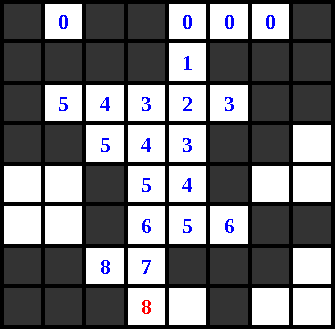
\includegraphics[width=0.5\textwidth]{wave.pdf}
\caption{\label{wave}水波探测算法}
\end{minipage}
\begin{minipage}[b]{.5\textwidth}
\centering
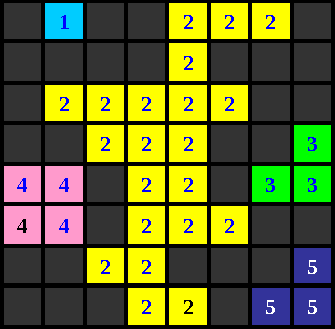
\includegraphics[width=0.5\textwidth]{hk.pdf}
\caption{\label{hk}Hoshen-Kopelman算法}
\end{minipage}
\end{figure}
然后可以通过一定量的计算测试, 比较各算法的优劣性(主要是时间复杂性), 以确定最终采用的算法. 下面先给出具体算法:
\begin{itemize}
\item 水波探测算法. 利用扩大波阵面的思想对渗透进行宽度搜索方式的探测. 图\ref{wave}说明了这一过程, 图中的数字表示每一步探测到的位置. 第一个波包含了网格第一行的所有开放位置. 根据图\ref{wave}所示, 第一个波包含了4个开放网格点, 并用`0'标记. 第二个波包含了除第一个波以外的所有位置, 并且可以由第一个波中一个位置一步到达. 通常, 第$k$个波是根据第$k-1$个波产生的, 它包含了之前不能到达的位置. 波从0开始, 且是有限的. 注意, 如果一个位置在 波$k$中出现, 则存在一条从第一行的一个位置开始长为$k$的路径. 因此, 水波探测算法不仅可以用来探测网格是否渗透, 而且还可以找到渗透的最短路径.
    图\ref{wave}中最终在第9个波后探测到通路.
\begin{table}[!htb]
\centering
\caption{\label{waveAlgorithm}水波探测算法伪代码}
{\tiny
\begin{tabular}{|lllllllll}
\hline
\multicolumn{9}{|l|}{The Wave Algorithm} \\
\hline
\multicolumn{5}{|l|}{\textbf{function} wave(grid)} & \multicolumn{4}{l|}{\textbf{function} gen\_wave(grid, current)} \\
 & \multicolumn{4}{l|}{n = size(grid); {~}next\_wave = []} &  & \multicolumn{3}{l|}{next  = [];} \\
 & \multicolumn{4}{l|}{\textbf{for} i \textbf{from} 1 \textbf{to} n} &  & \multicolumn{3}{l|}{\textbf{for} row, col \textbf{in} current} \\
 &  & \multicolumn{3}{l|}{\textbf{if} grid(1,i) == 1 \textbf{then}} &  &  & \multicolumn{2}{l|}{wave = grid(row, col) + 1} \\
 &  &  & \multicolumn{2}{l|}{grid(1,i) = 2} &  &  & \multicolumn{2}{l|}{\textbf{if} row+1$<$n \textbf{and} grid(row+1,col) ==1 \textbf{then}} \\
 &  &  & \multicolumn{2}{l|}{append(next\_wave, (1,i))} &  &  &  & \multicolumn{1}{l|}{grid(row+1,col) = wave; append(next, (row+1,col))} \\
 &  & \multicolumn{3}{l|}{\textbf{end\{if\}}} &  &  & \multicolumn{2}{l|}{\textbf{end\{if\}}} \\
 & \multicolumn{4}{l|}{\textbf{end\{for\}}} &  &  & \multicolumn{2}{l|}{\textbf{if} row-1>0 \textbf{and} grid(row+1,col) ==1 \textbf{then}} \\
 & \multicolumn{4}{l|}{\textbf{while} next\_wave} &  &  &  & \multicolumn{1}{l|}{grid(row-1,col) = wave; append(next, (row-1,col))} \\
 &  & \multicolumn{3}{c|}{next\_wave = gen\_wave(grid, next\_wave)} &  &  & \multicolumn{2}{l|}{\textbf{end\{if\}}} \\
 & \multicolumn{4}{l|}{\textbf{end\{while\}}} &  &  & \multicolumn{2}{l|}{\textbf{if} col+1< n \textbf{and} grid(row,col+1) ==1 \textbf{then}} \\
 & \multicolumn{4}{l|}{\textbf{for} i \textbf{from} i \textbf{to} n} &  &  &  & \multicolumn{1}{l|}{grid(row,col+1) = wave; append(next, (row,col+1))} \\
 &  & \multicolumn{3}{l|}{\textbf{if} grid(n, i) > 1 \textbf{then}} &  &  & \multicolumn{2}{l|}{\textbf{end\{if\}}} \\
 &  &  & \multicolumn{2}{l|}{ \textbf{return} true} &  &  & \multicolumn{2}{l|}{\textbf{if} col-1>0 \textbf{and} grid(row,col-1) ==1 \textbf{then}} \\
 &  & \multicolumn{3}{l|}{\textbf{end\{if\}}} &  &  &  & \multicolumn{1}{l|}{grid(row,col-1) = wave; append(next, (row,col-1))} \\
 & \multicolumn{4}{l|}{\textbf{end\{for\}}} &  &  & \multicolumn{2}{l|}{\textbf{end\{if\}}} \\
 & \multicolumn{4}{l|}{\textbf{return} false} &  & \multicolumn{3}{l|}{\textbf{end\{for\}}} \\
\multicolumn{5}{|l|}{\textbf{end\{function\}}} & \multicolumn{4}{l|}{\textbf{end\{function\}}} \\
\hline
\end{tabular}
}
\end{table}

\item 深度搜索算法. 一条通过网格的路径由新发现的位置和接下来最近发现的位置组成. 一旦发现被跟踪的路径进入死胡同, 则回溯到最近的一条没有探测过的分支, 并继续跟踪. 从某种意义上来讲, 这种方法与水波探测方法是相反的, 水波探测是针对整个网格一波接一波进行的.
\begin{table}[!htb]
\caption{深度搜索算法伪代码}
\centering{\scriptsize
\begin{tabular}{|lllll}
\hline
\multicolumn{5}{|l|}{The Recursive Algorithm} \\
\hline
\multicolumn{5}{|l|}{\textbf{function} Recursive(grid)} \\
 & \multicolumn{4}{l|}{n = size(grid)} \\
 & \multicolumn{4}{l|}{\textbf{for} i \textbf{from} 1 \textbf{to} n} \\
 &  & \multicolumn{3}{l|}{\textbf{if} explore(grid, 1, i) \textbf{then}} \\
 &  &  & \multicolumn{2}{l|}{\textbf{return} true} \\
 &  & \multicolumn{3}{l|}{\textbf{end\{if\}}} \\
 & \multicolumn{4}{l|}{\textbf{end\{for\}}} \\
 & \multicolumn{4}{l|}{\textbf{return} false} \\
\multicolumn{5}{|l|}{\textbf{end\{function\}}} \\
\hline
\multicolumn{5}{|l|}{\textbf{function} explore(grid, row, col)} \\
 & \multicolumn{4}{l|}{n = size(grid)} \\
 & \multicolumn{3}{l}{\textbf{if} grid(row,col)==1 \textbf{then}} & \multicolumn{1}{l|}{} \\
 &  & \multicolumn{3}{l|}{grid(row,col) = -1\textcolor{blue}{//给扫描过的位置贴上-1的标签}} \\
 &  & \multicolumn{3}{l|}{\textbf{if} row+1==n \textbf{then}} \\
 &  &  & \multicolumn{2}{l|}{\textbf{return} true} \\
 &  & \multicolumn{3}{l|}{\textbf{end\{if\}}} \\
 &  & \multicolumn{3}{l|}{\textbf{if} row+1$<$n \textbf{and} grid(row+1, col)==1 \textbf{then} explore(grid, row+1, col) \textbf{end\{if\}}} \\
 &  & \multicolumn{3}{l|}{\textbf{if} \hspace{0.5em}col+1$<$n \textbf{and} grid(row,\hspace{0.1em} col+1)==1 \textbf{then} explore(grid, row,\hspace{0.1em} col+1) \textbf{end\{if\}}} \\
 &  & \multicolumn{3}{l|}{\textbf{if} \hspace{0.4em}row-1$>$0 \textbf{and} grid(row-1, \hspace{0.3em}col)==1 \textbf{then} explore(grid,  \hspace{0.1em}row-1, \hspace{0.1em}col) \textbf{end\{if\}}} \\
 &  & \multicolumn{3}{l|}{\textbf{if}\hspace{0.9em} col-1$>$0 \textbf{and} grid(row, \hspace{0.4em}col-1)==1 \textbf{then} explore(grid, row-1, \hspace{0.2em}col) \textbf{end\{if\}}} \\
 & \multicolumn{4}{l|}{\textbf{end\{if\}}} \\
\multicolumn{5}{|l|}{\textbf{end\{fucntion\}}} \\
\hline
\end{tabular}}
\end{table}
\item Hoshen-Kopelman算法.给每一个开放网格贴一个标签. 同一个集群的网格标上相同的标签, 如图\ref{hk}所示.
 HK算法扫描网格时, 每扫到一个网格, 检查一下当前网格有没有已经被扫描过的邻居网格, 如果有邻居网格且都为阻碍网格, 则给当前网格标一个之前从没用过的标签, 以表示它属于一个新的集群. 如果只有一个邻居网格为开放网格, 则当前网格与该邻居标相同的标签, 如果有一个以上的邻居为开放网格, 它们的标签各不相同, 则当前网格标其邻居标签中较小的一个. 当然, 相邻的网格, 若标有不同的标签, 它们将在重新标注时标成相同的标签, 以表示它们属于同一集群. 显然Hk算法不仅可以通过查找首尾行有没有相同的标签来判断是否发生渗透, 还可以给出最大集群.
\begin{table}[!htb]
\centering
\caption{Hoshen-Kopelma的伪代码}{\scriptsize
\begin{tabular}{|llllllllll|}
\hline
\multicolumn{10}{|l|}{The Hoshen-Kopelman Algorithm} \\
\hline
 & \multicolumn{9}{l|}{largest\_label = 0} \\
 & \multicolumn{9}{l|}{\textbf{for} i \textbf{from} 1 \textbf{to} n} \\
 &  & \multicolumn{8}{l|}{\textbf{for} j \textbf{from} 1 \textbf{to} n} \\
 &  &  & \multicolumn{7}{l|}{ \textbf{if} grid(i,j) == 1 \textbf{then}} \\
 &  &  &  & \multicolumn{6}{l|}{left = grid(i-1,j); {~}above = grid(i,j-1)} \\
 &  &  &  & \multicolumn{6}{l|}{ \textbf{if} left == 0  \textbf{and} above == 0  \textbf{then}} \\
 &  &  &  &  & \multicolumn{5}{l|}{largest\_label = largest\_label + 1 } \\
 &  &  &  &  & \multicolumn{5}{l|}{label(i,j) = largest\_label} \\
 &  &  &  & \multicolumn{6}{l|}{ \textbf{else}} \\
 &  &  &  &  & \multicolumn{5}{l|}{ \textbf{if} left $\neq$ 0  \textbf{then}} \\
 &  &  &  &  &  & \multicolumn{4}{l|}{ \textbf{if} above $\neq$ 0  \textbf{then}} \\
 &  &  &  &  &  &  & \multicolumn{3}{l|}{union(left, above)\textcolor{blue}{//left和above属于相同的集群, 标相同标签{~~~~}}} \\
 &  &  &  &  &  & \multicolumn{4}{l|}{\textbf{end\{if\}}} \\
 &  &  &  &  &  & \multicolumn{4}{l|}{label(i,j) = find(left)\textcolor{blue}{//找出left所属的集群} } \\
 &  &  &  &  & \multicolumn{5}{l|}{ \textbf{else}} \\
 &  &  &  &  &  & \multicolumn{4}{l|}{label(i,j) = find(above)} \\
 &  &  &  &  & \multicolumn{5}{l|}{ \textbf{end\{if\}}} \\
 &  &  &  & \multicolumn{6}{l|}{ \textbf{end\{if\}}} \\
 &  & \multicolumn{8}{l|}{ \textbf{end\{for\}}} \\
 & \multicolumn{9}{l|}{ \textbf{end\{for\}}} \\
\hline
\end{tabular}}
\end{table}
\end{itemize}
需要注意的是, 为了叙述的方便, 上面提供的算法描述, 伪代码及附录提供的程序这三者间略有差异.
\section{结果}
本文对系统尺度$n$为10, 25, 50, 75, 100的五种情况分别进行了计算实验. 通过1000次的初步计算: 发现当开放概率$p\in[0,0.15]$及$p\in[0.85,1.0]$时, 各系统发生渗透的概率为0, 因此这两个区间内无需再作计算; 各情况下渗透概率在$[0.5, 0.7]$区间内发生突变, 因此该区间内需要较细致的计算. 另外, 分别对三种算法的性能进行了测试: 发现同一种算法下, 单次渗透实验完成所需时间不仅与系统尺度$n$有关, 还与点开放概率有关, 系统尺度为10, 25, 50 和100四种情况下三种算法单次渗透实验完成所需时间随点开放概率的变化曲线分别如图\ref{size10}-\ref{size100}.
\begin{figure}[!htb]
\begin{minipage}[b]{.5\textwidth}
\centering
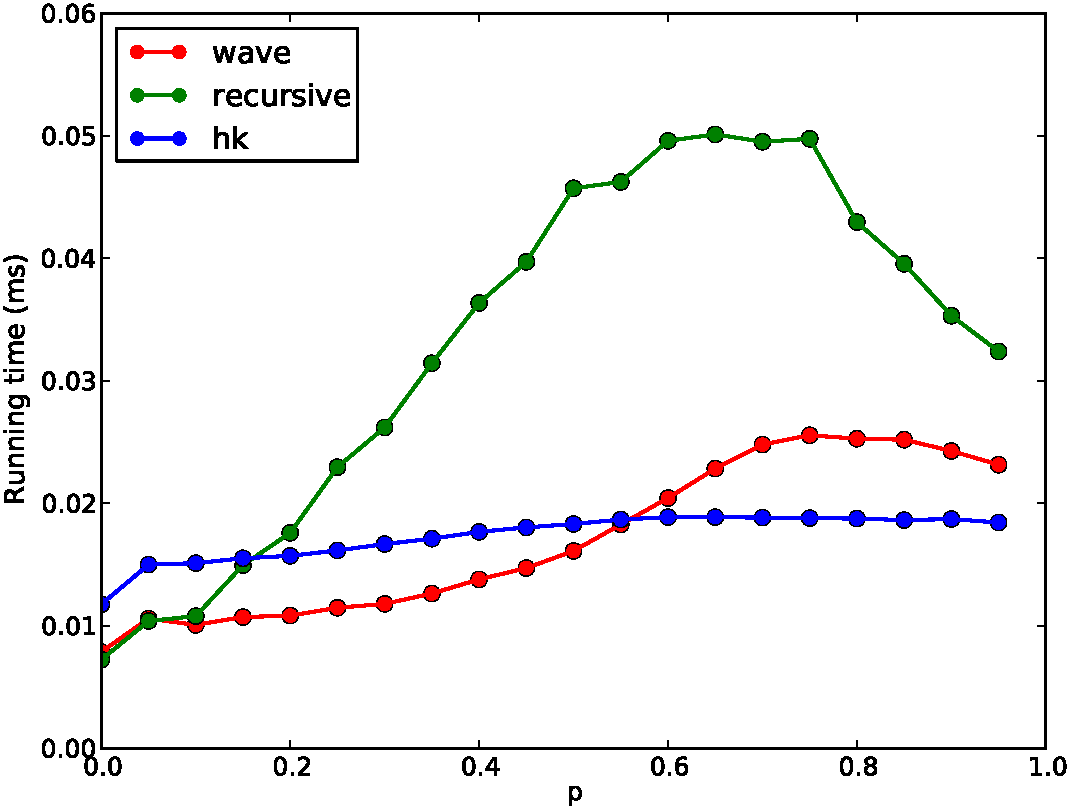
\includegraphics[width=0.9\textwidth]{10.pdf}
\caption{\label{size10}系统尺度为10三种算法运行时间}
\end{minipage}
\begin{minipage}[b]{.5\textwidth}
\centering
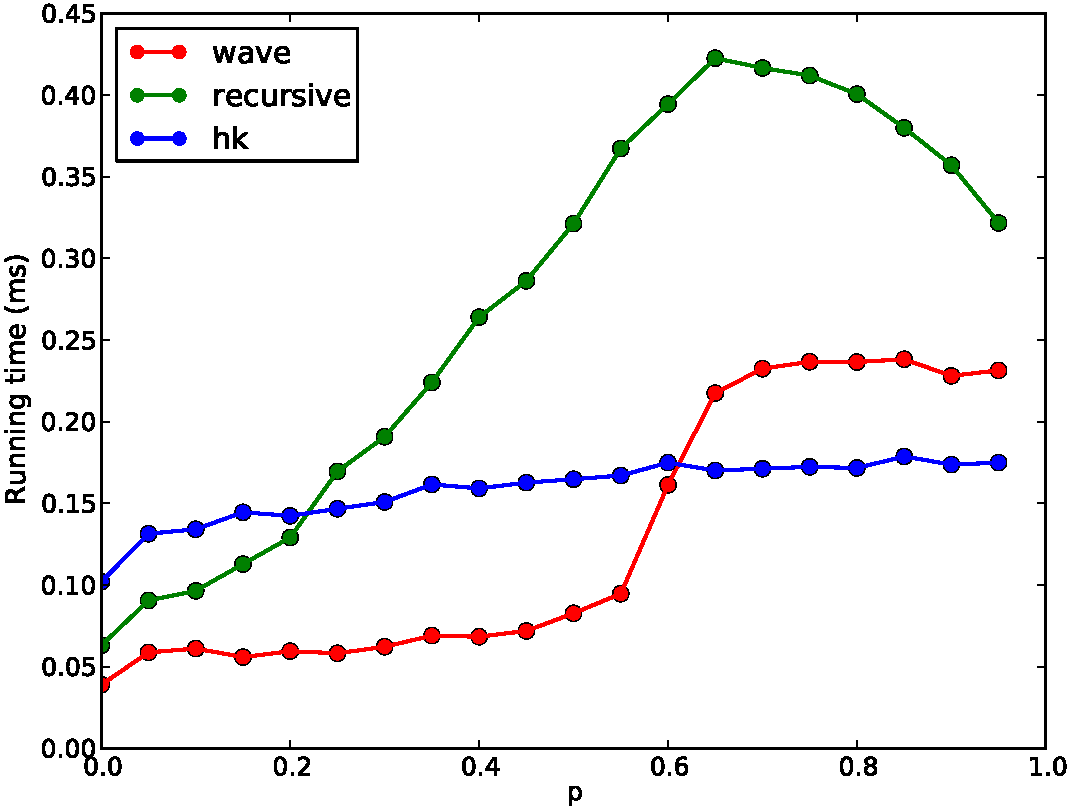
\includegraphics[width=0.9\textwidth]{25.pdf}
\caption{\label{size25}系统尺度为25三种算法运行时间}
\end{minipage}
\end{figure}
\begin{figure}[!htb]
\begin{minipage}[b]{.5\textwidth}
\centering
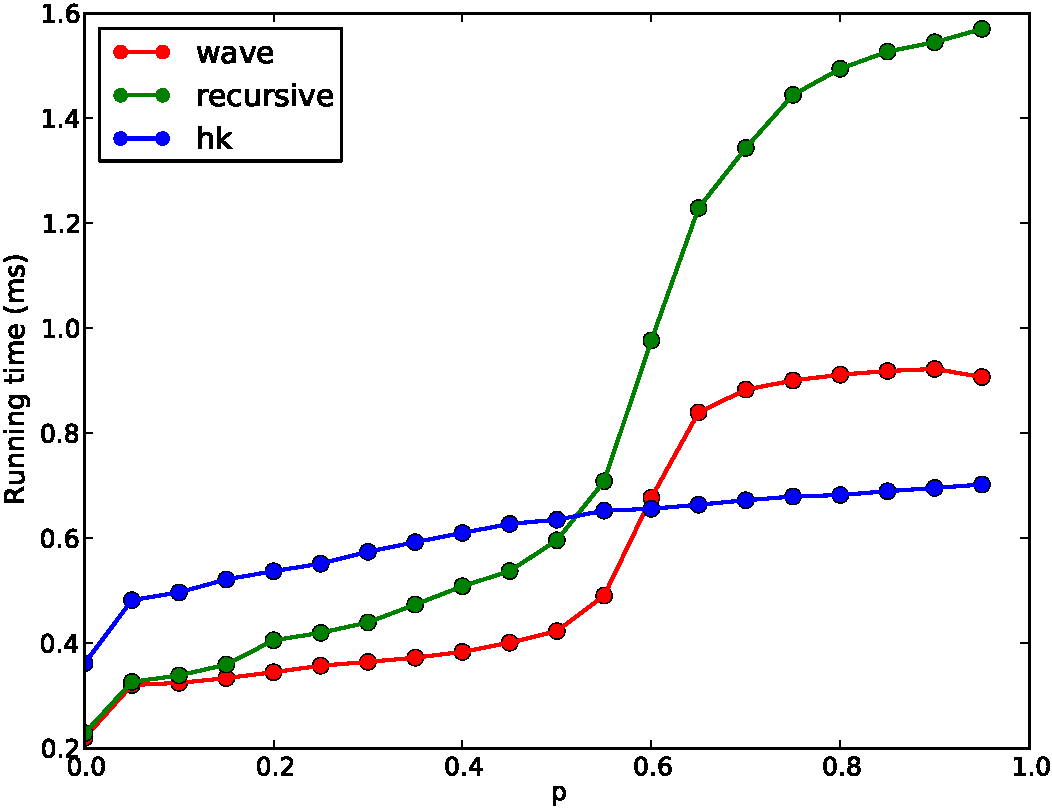
\includegraphics[width=0.92\textwidth]{50.pdf}
\caption{\label{size50}系统尺度为50三种算法运行时间}
\end{minipage}
\begin{minipage}[b]{.5\textwidth}
\centering
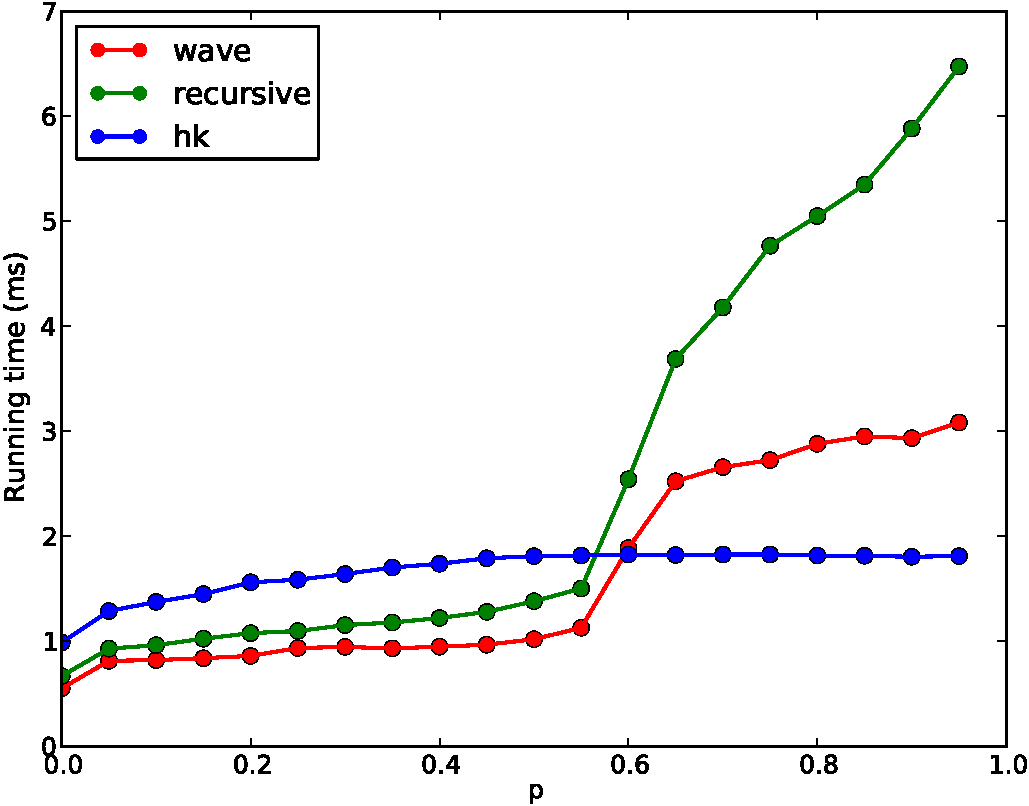
\includegraphics[width=0.9\textwidth]{100.pdf}
\caption{\label{size100}系统尺度为100三种算法运行时间}
\end{minipage}
\end{figure}
可以看出:
水波探测算法完成一次实验的耗时曲线比较有意思, 好像也存在相变, 且相变点的概率与后面得到的系统相变的概率几乎相同, p在区间[0,0.5]及[0.7, 1.0]分别较缓慢增长, 在[0.5,0.7]上发生了急剧上升; 深度搜索算法在系统尺度较小时($n=10,25$)的耗时曲线先增加后减小, 最大耗时点约为0.6, 也在相变点附近. 在系统尺度较大时($n=50,100$)的耗时曲线先缓慢增加后快速增加;
HK算法在不同尺度下, 耗时曲线随$p$增长缓慢. 比较三个算法, 可以发现各系统尺度下, 点开放概率较小时($<0.6$)水波探测算法最好; 当点开放概率较大时($>0.6$), Hk算法最好; 各情况下, 深度搜索算法在三种算法中都表现较差. 基于上述分析, 本文对之后更为细致的计算进行了如下调整:
\begin{itemize}
\item 系统点开放概率在0.6以下的由水波探测算法计算; 系统点开放概率在0.6及0.6以上的由HK算法计算.
\item 只计算点开放概率在区间$[0.15,{~}0.85]$, 0.15以下, 0.85以上的渗透概率直接赋0.
\item 点开放概率$p$在区间$[0.15,{~}0.5]$及$[0.7,{~}0.85]$每隔0.02计算一次; 在$[0.5, 0.7]$每隔0.005计算一次.
\end{itemize}
本文对于每种尺度下每种点开放概率的渗透实验, 分别进行了$2\times10^5$次的计算, 然后用发生渗透的次数除以计算的总次数得到渗透的概率. 最终结果如图\ref{prob1}和图\ref{prob2}所示(图\ref{prob2}是图\ref{prob1}相变概率附近局部区域的放大图).
\begin{figure}[!htb]
\begin{minipage}[b]{.5\textwidth}
\centering
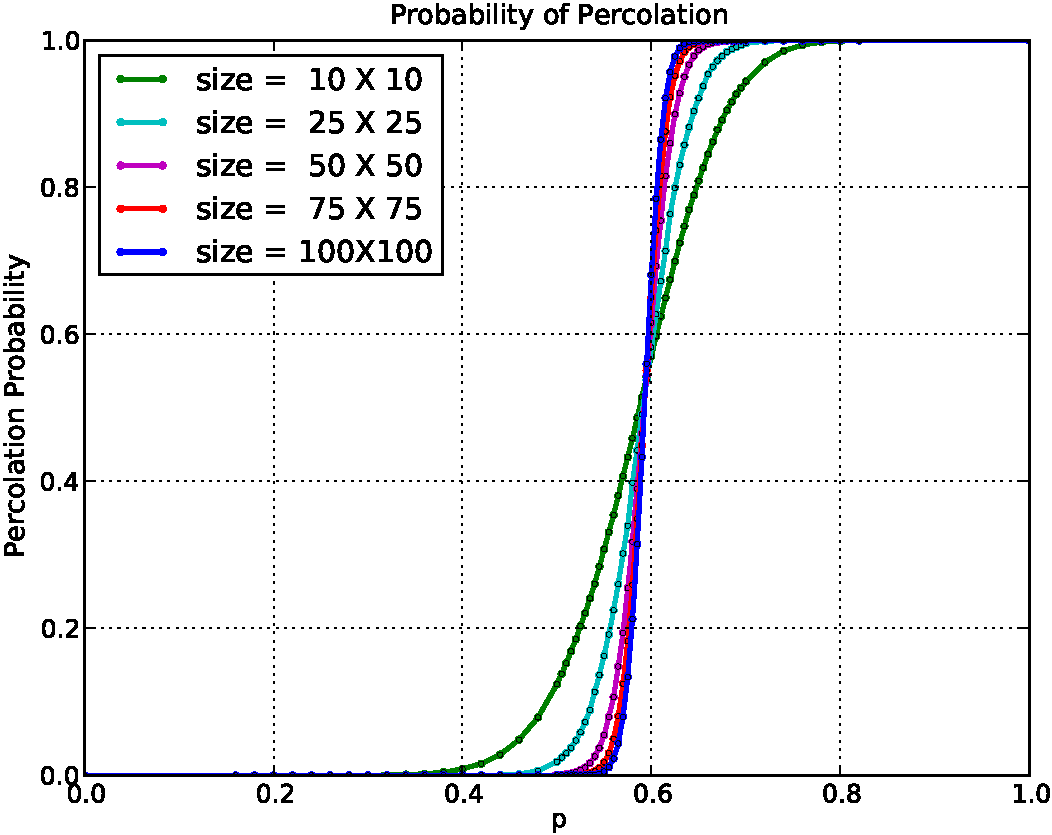
\includegraphics[width=0.9\textwidth]{prob1.pdf}
\caption{\label{prob1}不同系统尺度各开放概率下的渗透概率}
\end{minipage}
\begin{minipage}[b]{.5\textwidth}
\centering
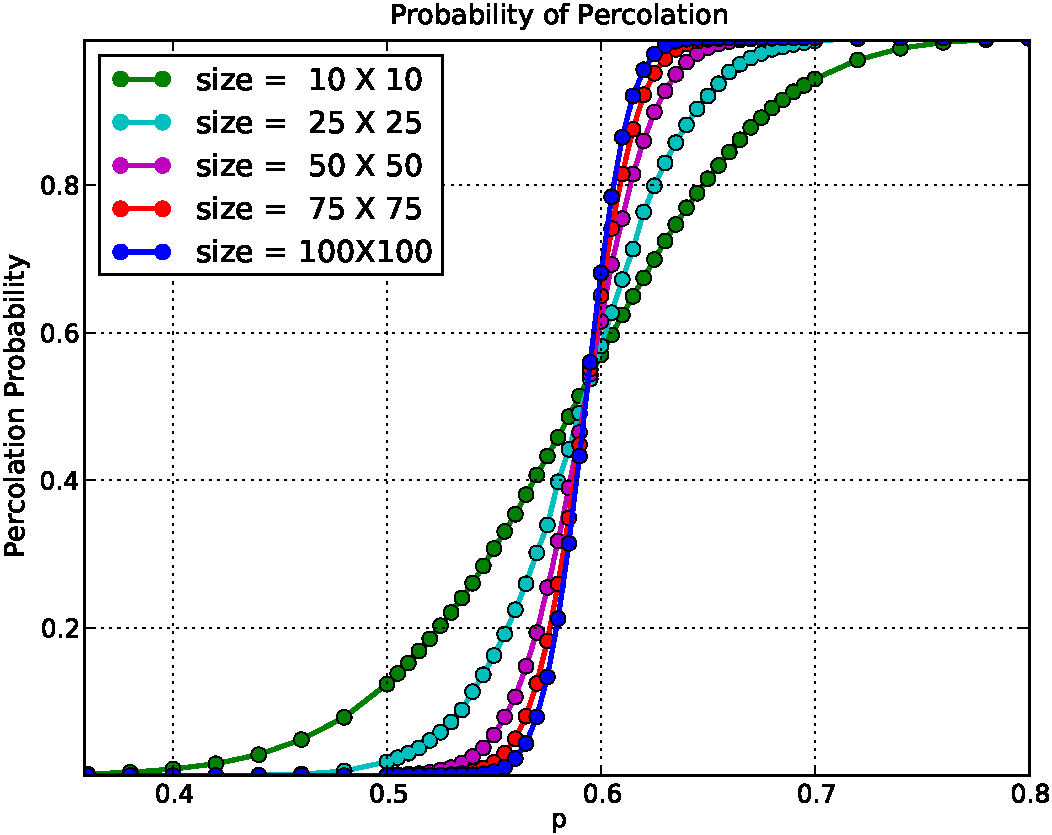
\includegraphics[width=0.9\textwidth]{prob2.pdf}
\caption{\label{prob2}渗透概率相变点附近的放大图}
\end{minipage}
\end{figure}
从图中可以看出, 各尺度下的渗透概率曲线约在$p=0.59$附近相交于一点. 因此可估计出$p_c$的值约为0.59左右.
同时还可以看出, 系统的尺度越大, 曲线在相变点附近突变的越剧烈, 可以用渗透概率曲线在相变点处的斜率衡量突变的剧烈程度, 也可以用渗透概率从$0^+$变化为$1^-$的平均斜率即
\[
\frac{\Delta q}{\Delta p} = \frac{1}{p|_{q=1^-} - p|_{q=0^+}}
\]
来衡量突变的剧烈程度. 根据计算所得到的数据, 容易得到图\ref{slope}所示的渗透概率曲线在相变点处的斜率及整个突变过程的平均斜率.
\begin{figure}[!htb]
\centering
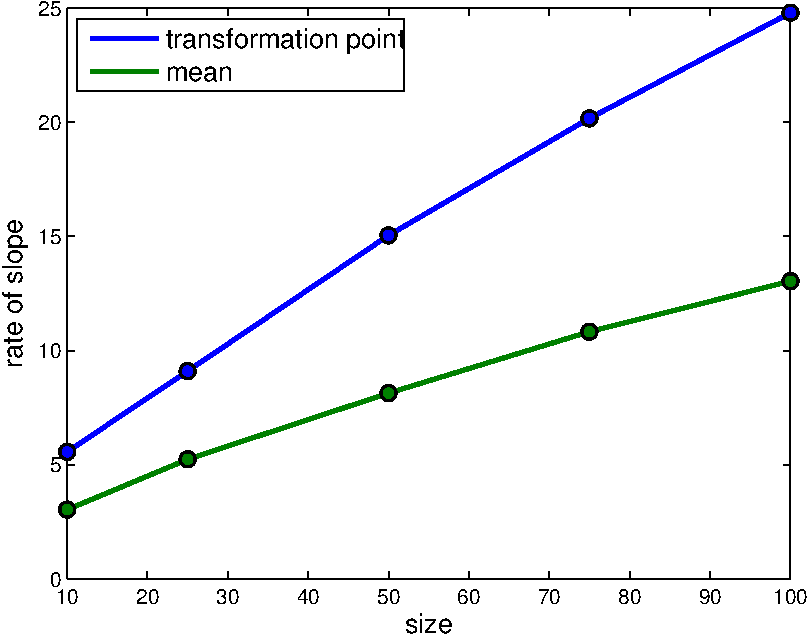
\includegraphics[width=0.5\textwidth]{slope.pdf}
\caption{\label{slope}渗透概率曲线在相变点处的斜率及整个突变过程的平均斜率}
\end{figure}
从图\ref{slope}可以看到, 渗透概率曲线在相变点处的斜率及整个突变过程的平均
斜率随系统尺度的增加而较均匀的增加. 由此, 不必进行计算, 而只需通过拟合插值便可得到其它系统尺度的渗透概率曲线.
\section{总结}

本文利用计算机成功的对二维渗透理论进行了随机计算模拟, 并得到了合理的结果: 相变点$p_c$在0.59左右. 另外, 本文在计算方面采取了多种有效降低计算成本的方法: 通过对初步计算结果的分析, 本文采取对相变附近细致计算, 非相变附近粗略计算或不计算, 使得在保证结果相当精细的前提下, 大大减少了不必要的计算;
同时, 本文还在不同条件下使用不同的算法, 大大减小了计算所需要的时间.



\begin{thebibliography}{99}
\bibitem{1} M Basta, V Picciarelli and R Stella. An introduction to percolation. Eur. J. Phys. 15 11994 97-101. Printed in the UK.
\bibitem{2} Percolation theory. http://en.wikipedia.org/wiki/Percolation\_theory
\bibitem{7} Union Find. http://www.cs.duke.edu/courses/cps100e/spring11/forbes/notes/UnionFind-4up.pdf
\bibitem{1} Percolation in Grids. http://secant.cs.purdue.edu/cs190c:project2\_09\\
    http://www.cnblogs.com/yuxc/category/296463.html
\bibitem{2} The Hoshen-Kopelman Algorithm. \\ http://www.ocf.berkeley.edu/\~fricke/projects/hoshenkopelman/hoshenkopelman.html

\end{thebibliography}


\newpage
\appendix
\appendixpage
\begin{subappendices}
\section{main\_percolation.py}
{\scriptsize
\begin{python}
"""
main_percolation.py: main script to test percolation system

Zhou Lvwen, zhou.lv.wen@gmail.com
Physical Simulation: project 01
"""
from percolation_wave import *
from percolation_recursive import *
from percolation_hk import *
from sys import *
step = 0.01
trial_count = 20
size = 20
p = 0
print 'Running for size =', size
data = open("percolation.data", 'w')
data.write("--------size = %d--------\n" %size)
data.write("Occupation \t spanning\n")
data.write("probability \t probability\n")
while p < 1:
    stdout.write("-")
    stdout.flush()
    perc_count = 0
    for k in range(trial_count):
        g = random_grid(size, p, 2)
        #flow,perc = percolation_wave(g)
        #flow,perc = percolation_recursive(g)
        flow,perc = percolation_hk(g)
        if perc:
           perc_count += 1

    prob = float(perc_count)/trial_count
    data.write("%f\t %f\n" % (p, prob))
    p += step
stdout.write(">|" + "\n")
data.close()
\end{python}
}
\section{main\_size\_varies.py}
\begin{python}
"""
main_size_varies.py: main script to test different size systems

Zhou Lvwen, zhou.lv.wen@gmail.com
Physical Simulation: project 01
"""
from percolation_wave import *
from percolation_recursive import *
from percolation_hk import *
from sys import *
step = 0.01
trial_count = 1000000
sizes = [10, 25, 50, 75, 100]

n = 0
results=[]
P = []
for size in sizes:
    p = 0.01
    results.append([])
    print 'Running for size =', size
    while p < 1:

        stdout.write("-")
        stdout.flush()

        perc_count = 0

        for k in range(trial_count):
            g = random_grid(size, p, 2)
            flow,perc = percolation_hk(g,True)
            if perc:
                perc_count += 1
            #endif
        #endfor
        prob = float(perc_count)/trial_count
        #print 'percolation q=',prob
        results[n].append(prob)
        P.append(p)
        p += step

    #endwhile
    stdout.write(">|" + "\n")
    n += 1
#endfor

data = open("percolation.data", 'w')
data.write("Occupation \t\t spanning probability\n")
data.write("probability \t")
for sizei in sizes:
    data.write("size ="+repr(sizei)+"\t")
#endfor
data.write("\n")

for i in range(len(results[0])):
    data.write("\n")
    data.write("%f\t" % P[i])
    for j in range(len(sizes)):
        data.write("%f\t" % results[j][i])
    #endfor
#endfor
data.close()
\end{python}

\section{main\_function\_time.py}
\begin{python}
"""
main_function_time.py: main script to test different functions

Zhou Lvwen, zhou.lv.wen@gmail.com
Physical Simulation: project 01
"""

from percolation_wave import *
from percolation_recursive import *
from percolation_hk import *
import time
import sys

step = 0.05
trial_count = 100000
size = 10

def test_time(func):
    p = 0
    results = []
    old_clock = time.clock()

    print 'testing', func, '...'

    while p < 1:

        perc_count = 0
        for k in range(trial_count):
            g = random_grid(size, p)
            flow,perc = func(g)
        new_clock = time.clock()
        results.append((new_clock - old_clock)*1000/trial_count)
        old_clock = new_clock
        p += step
        sys.stdout.write("-")
        sys.stdout.flush()
    sys.stdout.write(">|\n")
    return results

if __name__ == '__main__':

    sys.setrecursionlimit(250000)

    res1 = test_time(percolation_wave)
    res2 = test_time(percolation_recursive)
    res3 = test_time(percolation_hk)
    data = open("funion10.time", 'w')
    data.write("Occupation \t wave fun \t recursive fun \t\n")
    data.write("probability \t time use\t time use\t\n")
    for i in range(len(res1)):
        data.write(("\n"+"%f\t"*4) % (step*i, res1[i], res2[i], res3[i]))
    #endfor
    data.close()
\end{python}

\section{Percolation\_hk.py}
\begin{python}
"""
Percolation_hk.py: Apply the Hoshen-Kopelman Algorithm for Cluster Spanning
Based on http://www.ocf.berkeley.edu/~fricke/projects/
                hoshenkopelman/hoshenkopelman.html

Zhou Lvwen, zhou.lv.wen@gmail.com
Physical Simulation: project 01
"""

from grid import *

def percolation_hk(input_grid, short=False):
    size = len(input_grid)
    for i in range(size):
        for j in range(size):
            input_grid[i][j] = 1 - input_grid[i][j]
    n_labels = 0 # number of labels used so far

    labels = [0]*(size*size)

    for i in range(size):
        for j in range(size):
            if input_grid[i][j] == 1:
               # check the neighbors of this cell, up and to the left
               up = 0;
               left = 0;
               if i>0 :
                  up = input_grid[i-1][j]
               if j>0 :
                  left = input_grid[i][j-1]

               if up==0 and left == 0: # new cluster
                  n_labels  = n_labels + 1
                  labels[n_labels] = n_labels
                  input_grid[i][j] = n_labels
               elif up==0 or left==0: # same cluster
                  input_grid[i][j] = max(up,left)
               else: # two clusters
                   # dereference the label until it points to itself
                   while labels[up]<up:
                       up = labels[up]
                   while labels[left]<left:
                       left = labels[left]
                   input_grid[i][j]=min(up,left)
                   labels[max(up,left)] = min(up,left)
    # Renumber the labels so that they're continuous, and eliminate
    # cluster aliases
    j = 0
    for i in range(n_labels):
        if labels[i]==i:
           labels[i] = j
           j+=1
        else:
           labels[i] = labels[labels[i]]
    # apply the relabeling to the input_grid
    for i in range(size):
        for j in range(size):
            input_grid[i][j] = labels[input_grid[i][j]]

    return input_grid, ifspanning(input_grid)

def ifspanning(input_grid):
    size = len(input_grid)
    n = 0
    label = max(input_grid[0])
    if label>0:
       for i in range(size):
            if input_grid[size-1][i] >0 and input_grid[size-1][i]<=label:
               return True
    return False
\end{python}

\section{Percolation\_recursive.py}
\begin{python}
"""
Percolation_recursive.py: Solve Cluster Spanning problem by Recursive
                          Exploration of the Grid
Based on http://secant.cs.purdue.edu/cs190c:project2\_09
         http://www.cnblogs.com/yuxc/category/296463.html

Zhou Lvwen, zhou.lv.wen@gmail.com
Physical Simulation: project 01
"""
from grid import *

def percolation_recursive(input_grid, short=False):
    """
    Determine whether or not a grid percolates, and which cells are filled.
    Like before, short is True if you want the algorithm to stop immediately
    when it percolates, rather than exploring the entire grid.
    """
    size = len(input_grid)
    flow_grid = grid(size, -1)

    #start exploration from each space in top (zeroth) row
    for col in range(size):
        if explore(input_grid, flow_grid, 0, col, short):
            return flow_grid, True

    #check last (size-1'th) row for full spaces
    for col in range(size):
        if flow_grid[size-1][col] == '*':
            return flow_grid, True

    #no full spaces in bottom row; doesn't percolate
    return flow_grid, False

def explore(input_grid, flow_grid, row, col, short):
    """Explore the grid, marking unblocked cells as full as they are
       explored"""

    size = len(input_grid)
    if input_grid[row][col] == 0:
        flow_grid[row][col] = '*'

        #explore neighboring cells

        if short:
            if row + 1 == size:
                return True

        # Look down
        if row + 1 < size:
            if input_grid[row+1][col] == 0 and flow_grid[row+1][col] == -1:
               explore(input_grid, flow_grid, row+1, col, short)
        # Look right
        if col + 1 < size:
            if input_grid[row][col+1] == 0 and flow_grid[row][col+1] == -1:
               explore(input_grid, flow_grid, row, col+1, short)
        # Look left
        if col - 1 >= 0:
            if input_grid[row][col-1] == 0 and flow_grid[row][col-1] == -1:
               explore(input_grid, flow_grid, row, col-1, short)
        # Look up
        if row - 1 >= 0:
            if input_grid[row-1][col] == 0 and flow_grid[row-1][col] == -1:
               explore(input_grid, flow_grid, row-1, col, short)
\end{python}

\section{Percolation\_wave.py}
\begin{python}
"""
Percolation_wave.py: Solve percolation using the idea of expanding
                     wavefronts.
Based on http://secant.cs.purdue.edu/cs190c:project2\_09
         http://www.cnblogs.com/yuxc/category/296463.html

Zhou Lvwen, zhou.lv.wen@gmail.com
Physical Simulation: project 01
"""
from grid import *

def percolation_wave(input_grid, short=False):
    """
    Percolation algorithm by wave. Uses input_grid to determine where
    flow is allowed, trace to determine whether or not to visualize it
    graphically, and short to determine whether or not to exit early.
    Essentially, if your algorithm exits early, the code inside the
    'if short' condition is what your code might look like.
    """
    flow_grid = grid(len(input_grid), -1)
    next_wave = []

    # Populate the inital wave from the top row
    for k in range(len(input_grid[0])):
        if input_grid[0][k] == 0:
            flow_grid[0][k] = 1
            next_wave.append((0,k))

    while next_wave:

        if short:
            row = len(flow_grid) - 1
            for k in range(len(flow_grid[0])):
                if flow_grid[row][k] != -1:
                    return flow_grid, True

        next_wave = gen_next_wave(input_grid, flow_grid, next_wave)

    # Check if we made it to the bottom
    row = len(flow_grid) - 1
    percolates = False
    for k in range(len(flow_grid[0])):
        if flow_grid[row][k] != -1:
            percolates = True

    return flow_grid, percolates

def gen_next_wave(input_grid, flow_grid, current):
    next = []

    for row, col in current:
        wave = flow_grid[row][col] + 1

        # Look down
        if row + 1 < len(input_grid):
            if input_grid[row+1][col] == 0 and flow_grid[row+1][col] == -1:
                flow_grid[row+1][col] = wave
                next.append((row+1, col))

        # Look right
        if col + 1 < len(input_grid[0]):
            if input_grid[row][col+1] == 0 and flow_grid[row][col+1] == -1:
                flow_grid[row][col+1] = wave
                next.append((row, col+1))

        # Look left
        if col - 1 >= 0:
            if input_grid[row][col-1] == 0 and flow_grid[row][col-1] == -1:
                flow_grid[row][col-1] = wave
                next.append((row, col-1))

        # Look up
        if row - 1 >= 0:
            if input_grid[row-1][col] == 0 and flow_grid[row-1][col] == -1:
                flow_grid[row-1][col] = wave
                next.append((row-1, col))

    return next
\end{python}
\end{subappendices}

\end{document}
